\documentclass[tikz,border=2pt]{standalone}
\usepackage{amsmath,amssymb}
\usepackage{tikz}
\usetikzlibrary{arrows.meta}

\begin{document}
% A cycle (tour): a path that returns to its starting vertex, using each edge at most once;
% here B-D-E-C-B.
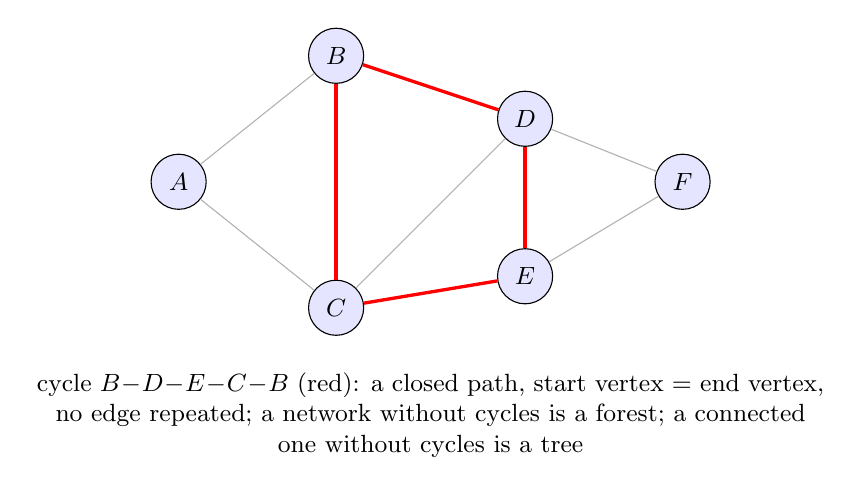
\begin{tikzpicture}[every node/.style={font=\small}, v/.style={draw, circle, fill=blue!10, minimum size=7mm, inner sep=0pt}]
	\node[v] (A) at (0,0) {$A$};
	\node[v] (B) at (2,1.6) {$B$};
	\node[v] (C) at (2,-1.6) {$C$};
	\node[v] (D) at (4.4,0.8) {$D$};
	\node[v] (E) at (4.4,-1.2) {$E$};
	\node[v] (F) at (6.4,0) {$F$};
	\foreach \a/\b in {A/B, A/C, C/D, D/F, E/F} {\draw[gray!60] (\a) -- (\b);}
	\draw[red, very thick] (B) -- (D);
	\draw[red, very thick] (D) -- (E);
	\draw[red, very thick] (E) -- (C);
	\draw[red, very thick] (C) -- (B);
	\node[anchor=north, align=flush center, text width=10cm] at (3.2,-2.3) {cycle $B\!-\!D\!-\!E\!-\!C\!-\!B$ (red): a closed path, start vertex = end vertex, no edge repeated; a network without cycles is a forest; a connected one without cycles is a tree};
\end{tikzpicture}
\end{document}
